\chapter{Across language boundaries}

We speak in many ways. Some of us use academic language for scholarly articles and academic settings with specialized terminology and formal structures differing significantly from our everyday conversations. At the same time, we recognize the similarities and differences between that and the precise and structured language of legal English, a form reflecting the often adversarial nature of law and an accumulated body of precedence.

Literary English showcases a broad spectrum of styles, from classical literature's elevated diction and meandering clause structure to the colloquialisms in contemporary works, and we traverse among them, usually unhampered by any linguistic borders. In film and television, writers combine colloquial speech with scripted language, accommodating a wide range of social contexts and character archetypes, the language differences evoking for us myriad elements of character and setting, at least when done well. 

Bill Withers moves us with the lamentation, \textit{ain't no sunshine when she's gone}, even though its grammatical structures might not be ones we typically use -- though we could if we would. We can even do dialectal time travel: somehow, even today, we know to avoid contractions when producing ``old'' English, reflecting a change that took place more than three centuries ago (Castillo González 2007). 

In poetry, too, are dances we do not elsewhere do. Advertising and marketing English is persuasive and catchy, often employing creative wordplay to appeal to diverse audiences. Sports commentary uses a specific set of terms unique to each sport, highlighting the dynamic nature of sports culture, and its idioms often enjoy something like home-field advantage in many non-sporting contexts.

The Scottish use of Scots, a Germanic language closely related to English, in conjunction with Standard English, showcases the kind of dual linguistic identity seen in many places. Singlish, a colloquial form of English in Singapore, amalgamates English with elements from Malay, Mandarin, and other Chinese dialects. Beyond these, there are the pidgins and creoles, where English blends with other languages in multilingual communities, reflecting a mix of linguistic heritages. Many of us are multilingual, sometimes frighteningly so.

\begin{center}-- --\end{center}

\noindent From the viewpoint of Standard English, only (\ref{ex:nobody-has-come}) is grammatical. The \mymark{!}{} marks (\ref{ex:ain't-nobody}) as belonging to a non-Standard English, and, as usual * means it's just ungrammatical: nobody speaks like that.
\ea\label{ex:nobody-has}
    \ea[]{\textit{Nobody has come to help us.}}\label{ex:nobody-has-come}
    \exmark{!}{Ain't nobody come to help us.}\label{ex:ain't-nobody}
    \ex[*]{\textit{Isn't nobody come to help us.}}\label{ex:isn't-nobody}
    \ex[*]{\textit{Hasn't nobody come to help us.}}\label{ex:hasn't-nobody}
    \z
\z

\noindent But what about from the perspective of Singlish or of African American Vernacular English?\footnote{I'll just call it \textsc{African American English} without ``vernacular''.} While I don't know of any studies on the point, surely speakers of Singlish and African American English have extensive exposure to Standard English, and, perhaps more importantly, the Standard varieties are generally perceived as being correct, while the non-standard varieties, or at least salient elements thereof, are stigmatized. As a result, it seems likely that from the perspective of non-Standard English, both Standard and their own non-Standard varieties are grammatical, while, from the point of view of Standard English, the non-Standard forms are mostly seen as ungrammatical.

\begin{figure}
    \centering
    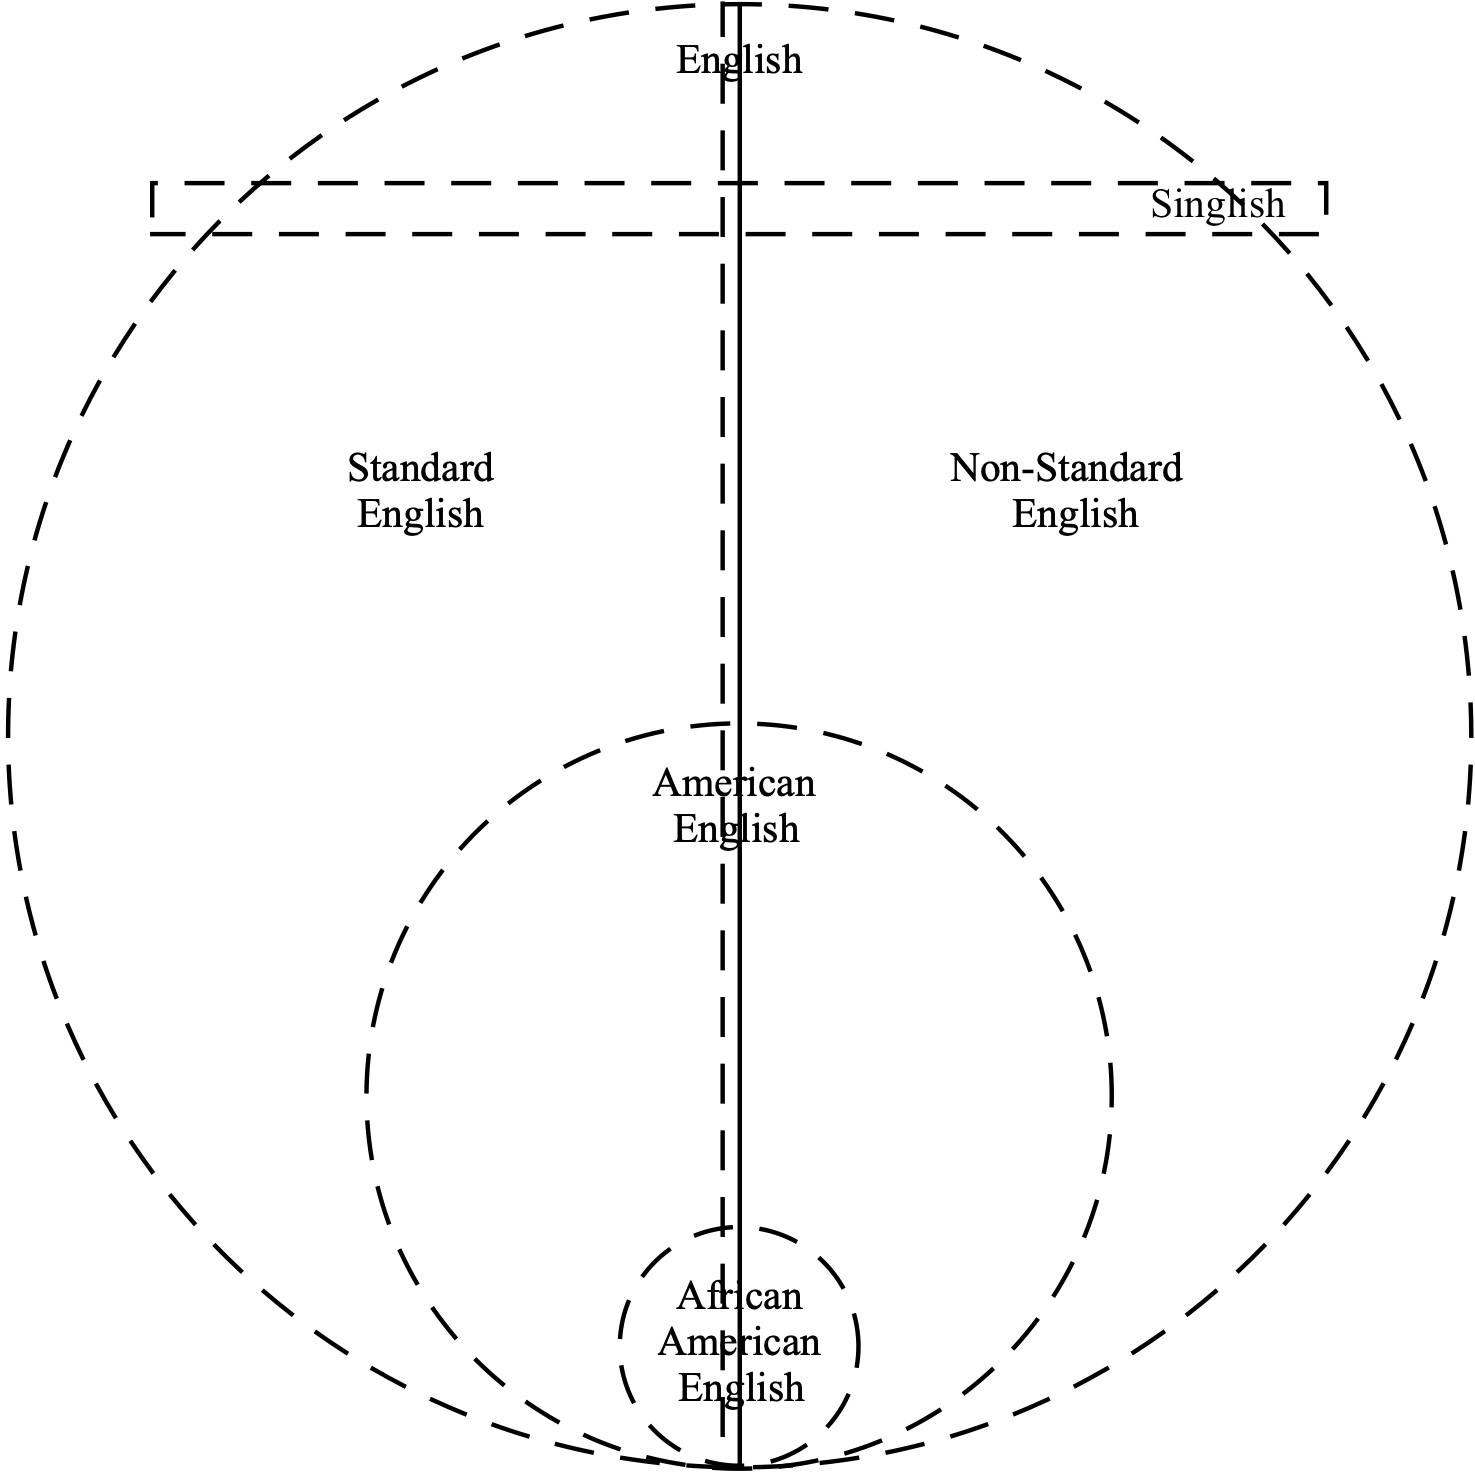
\includegraphics[width=0.8\textwidth]{figures/EnglishesVenn.png}
    \caption{The relationships among various varieties of English. Dotted lines show a certain permeability, while the solid vertical line shows that non-Standard forms are less readily accepted from the perspective of the Standard forms.}
    \label{fig:enter-label}
\end{figure}

If a Singlish speaker said, \textit{This person's Singlish is very good,} it would be considered grammatical in both Singlish and Standard English. If they said, \textit{This guy Singlish damn good leh,} that would still be grammatical in Singlish, but not in Standard English. And the non-Singlish Speaker might not even judge \textit{Wah lau! This guy Singlish si beh hiong sia} to be English, let alone have an opinion on its grammaticality.\footnote{The examples are taken from the Singlish article on \href{https://en.wikipedia.org/w/index.php?title=Singlish&oldid=1187889537}{\textit{Wikipedia}}.}

There are constructions such as (\ref{ex:isn't-nobody}) that are ungrammatical in any dialect. And then, there are those like (\ref{ex:ain't-nobody}), which are not only ungrammatical in Standard English but highly stigmatized, despite being grammatical in other varieties.  But there are also non-Standard constructions like (\ref{ex:BIN-living}), which are camouflaged \citep{Spears2015}. A Standard-English speaker might take it to be (\ref{ex:been-living}) and ignore it.

. 

\ea
    \eamark{!}{They've BIN living in Chicago.} \label{ex:BIN-living}
    \ex[]{\textit{They've been living in Chicago.}} \label{ex:been-living}
    \z
\z

But (\ref{ex:BIN-living}) isn't (\ref{ex:been-living}). Where \textit{they've been} could be any length of time, \textit{they've BIN} can only mean `for a long time' \citep{Spears2015}. This shows that, for something to be judged ungrammatical, it's needs to be noticed.

\begin{quote}
    In the all-Black schools I attended, for example, stigmatized vernacular language
features elicited reprimand and sometimes punitive measures. Even students, during all-student gatherings, regimented the language of other students to conform to the student “standard,” which tolerated a small set of vernacular forms (e.g., ain’t and multiple negatives). Even students, who today might be labeled thugs or gang members,13 participated in language policing, upbraiding or ridiculing peers for using habitual be, aks (cp. ask), or pronunciations considered to diverge too far from the standard norm. \cite[796]{Spears2015}
\end{quote}

\subsection{Just how different is it?}

The example in (\ref{ex:ain't-nobody}) likely feels familiar to you, and no doubt \textit{ain't} says clearly, ``this is not Standard English,'' which is true, as far as it goes. But it doesn't go nearly far enough. The next step is to notice that the Standard English construction employs \textit{have}, not \textit{be}, which is what we normally associate with \textit{ain't}.

A third departure is the location of the subject \textit{nobody}. In most English sentences, the subject precedes a verb, whether it be \textit{ain't} (\textit{\myuline{I} ain't eatin' that}) or something else. The major exception to this is in questions, such as \textit{Is \myuline{it} OK?}, where the subject swaps places with the auxiliary verb. Nothing about (\ref{ex:ain't-nobody}), though, would allow this kind of inversion in Standard English. 

Finally, both \textit{ain't} and \textit{nobody} are negatives. Now, despite what you may have been told, having two negatives in a sentences is perfectly normal in the world's languages (see \S\ref{sec:double-negs}). In Standard Italian, we find


\ea[]{
    \gll \textit{Non} \textit{è} \textit{venuto} \textit{nessuno} \textit{ad} \textit{aiutarci}\\
    not is come nobody to help-us \\
    \trans `Nobody came to help us.'
}
\z

But even though it's logically possible, it's still ungrammatical in Standard English. In those first two words alone, there are four grammatical differences between \textit{Ain't nobody come to help us} and \textit{Nobody has come to help us}.


%\subsection{Existential vs inversion}

%\ea
%    \eamark{!}{Ain't nothing like a beautiful sunrise to start the day.}
%    \exmark{!}{Don't everybody get a medal.}
%    \z
%\z
%\newpage
\section{Grammar in bilingual speech}

We've been considering the implications of using Standard vs non-Standard language, but that's far from exhausting the possibilities. When bilinguals speak amongst themselves, they often draw on both languages. By this point, you may not be surprised to find that there seem to be grammatical and ungrammatical ways to do this. 

Consider the position of adjectives. German syntax typically places adjectives (underlined) before the noun, as in \textit{eine \myuline{glückliche} Frau}  (`a \myuline{happy} woman'). In contrast, Italian favors post-nominal adjectives, yielding \textit{una donna \myuline{felice}}. This might suggest that, either order would be possible, but that's not the case. \textit{Una \myuline{glückliche} Frau} is grammatical for German--Italian bilinguals, but \textit{i \myuline{verdi} Augen} (`the green eyes'), for instance, is not \citep{Cantone2009}. 

I won't try to generalize from these two examples. The data seems inconsistent, and various positions have been staked out and defended (it depends on the language of the adjective!). Suffice it to say that independent bilingual speakers and communities across a range of language pairs have a surprising level of agreement on what is and what is not grammatical. It's not perfectly consistent, but it is predictable: there's a grammar behind it.

\begin{figure}
    \centering
    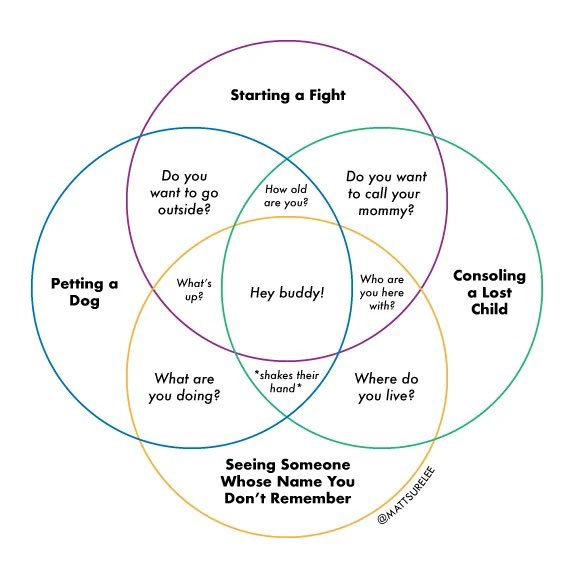
\includegraphics[width=0.8\textwidth]{figures/GAbtokpXgAAJYL0.jpg}
    \caption{A Venn diagram by Matt Shirley showing the contextual factors behind many simple expressions.}
    \label{fig:context-expressions}
\end{figure}

\section{One language, multiple grammars}
            \textit{Balinese}
        \begin{enumerate}
            \item \textsc{Intentionality}
            \item \textsc{Clarity}
            \item \textsc{Familiarity}
            \item \textsc{Group attitudes towards novelty}
            \item \textsc{Ideas of propriety}
            \item \textsc{Status maintenance}
        \end{enumerate}

\section{Gendered language}

Even as far back as 1944, \citet{Furfey1944} observed that men and woman had characteristically different ways of speaking. He cited expression like \textit{Oh, dear!} and \textit{How perfectly sweet!} as being feminine coded. Today, those might also feel a little dated, but we still have gender-coded language. I expect you have no problem determining which of the following are associated wither which gender.

\ea
    \ea[]{\textit{I feel so blessed!}}
    \ex[]{\textit{I'm stoked for this.}}
    \ex[]{\textit{I need to get laid.}}
    \ex[]{\textit{Isn't that adorable?}}
    \ex[]{\textit{Man up!}}
    \ex[]{\textit{Oh my gosh!}}
    \ex[]{\textit{Sick, dude!}}
    \ex[]{\textit{That's so sweet \op of you\cp.}}
    \z
\z

The question is, is your feeling upon hearing a masculine person say \textit{Oh my gosh!} fundamentally the same as when you hear an Anglophone say \textit{I no like that}? Each presents a mismatch between the persona and the signal encoded in the language. One is a gender mismatch, while the other is a competence mismatch. But is the competence mismatch somehow special?

\section{Microdialects}


In the early 1950s, two graduate students at Catholic University set out to study the dialect of African American residents living in the inhabited alleys of Washington D.C. Father George N. Putnam and Sister Rosina O'Hern were students of the sociologist Rev. Paul Hanly Furfey, who had introduced them to the field of the sociology of language.\footnote{I got this story from \citet[121--122]{Joseph2002}.}

The alleys, with their substandard living conditions, had for decades formed insular communities that developed their own distinctive linguistic features. Putnam and O'Hern interviewed 74 of the 88 known adult alley residents, carefully transcribing their speech phonetically. They also made tape recordings of five residents reading sentences and identifying objects, and even recounting one of \textit{Aesop's Fables}. 

The researchers subjected these recordings to detailed phonetic and spectrographic analysis, examining vowel and consonant qualities, stress, intonation and timing. They also noted non-standard grammar and vocabulary used by the residents based on the interviews and recordings.

But Putnam and O'Hern took things a step further with an innovative experiment. They recorded twelve African American speakers, three from the alleys and nine of higher social status, all telling the same story. They then played these recordings to 70 listeners and asked them to rank the speakers by social status. Remarkably, the rankings correlated very closely with the actual status of the speakers, showing that dialect alone, even in the absence of any other cues, strongly signaled social standing.

This study, published in 1955 in the journal \textit{Language}, demonstrated that we all track innumerable linguistic features, assigning all kinds of non-linguistic meanings to them. It's not likely that the judges had met or heard any residents of these alleys, so they would not have been able to form associations between their particular linguistic features and their socio-economic status. 

To the extent that we can trust their data,\footnote{``Labov perhaps not inaccurately but surely incompletely characterized'' it as unsystematic, saying ``and it is not clear what the judges were reacting to, or how representative their judgements were. (Labov 1966:19)'' as cited in \citet[125]{Joseph2002}.} this means that it must have been the residents themselves who extrapolated from the differences they observed in the language around them, subconsciously applying them to their own speech in ways that reflected their self perceptions of their place in society. And they must have done this in ways that resonated for the judges. This is a truly remarkable feat of coordination, one that likely benefits from innate attention to various linguistic and social factors, but not one that relies on any ``Universal Grammar''.